%%% Стилевой файл Вестника. Не изменять!
\documentclass[12pt,a4paper,twoside]{article}  %MikTeX
\usepackage[utf8]{inputenc}%Win
\usepackage[T1,T2A]{fontenc}
\usepackage{amsmath,amsfonts,amssymb,amscd,euscript}
\usepackage[english, russian]{babel}

\usepackage{graphicx}
\usepackage{psfrag}
\usepackage{cite}
\usepackage{caption}
\captionsetup[figure]{labelfont={bf},labelformat={default},labelsep=period,name={Рис.}}
\captionsetup[table]{labelfont={bf},labelformat={default},labelsep=period,name={Таблица}}

\usepackage[textwidth=166mm,top=2cm,textheight=250mm,left=20mm,showframe=false]{geometry}
\tolerance=500
\voffset=0.5cm
%\headsep=5mm
%\textwidth=166mm
%\textheight=250mm
%\oddsidemargin=-4mm
%\evensidemargin=-4mm
%\topmargin=-7mm

\usepackage{ifthen}
\newcommand{\serieseng}{\ifthenelse{\equal{МАТЕМАТИКА}{\seriesrus}}{MATHEMATICS}{\ifthenelse{\equal{МЕХАНИКА}{\seriesrus}}{MECHANICS}{\ifthenelse{\equal{КОМПЬЮТЕРНЫЕ НАУКИ}{\seriesrus}}{COMPUTER SCIENCE}{UNDEFINED}}}}

\makeatletter

\global\let\@fundingrus\@empty
\def\fundingrus#1{\gdef\@fundingrus{\@ifempty{#1}{\@empty}{\noindent{\bf Финансирование.} #1}}}

\global\let\@fundingeng\@empty
\def\fundingeng#1{\gdef\@fundingeng{\@ifempty{#1}{\@empty}{\noindent{\bf Funding.} #1}}}

%информация о статье на русском языке
\def\titlerus{\begin{otherlanguage}{russian}\thispagestyle{firstpagestylerus}\label{paperfirstpage}
		\hbox{УДК \UDC} \vspace{30pt plus 6pt}
		\begin{flushleft}
			{\bf\copyright~{\textit{\authorsrus}}\\[2ex]
				{\MakeUppercase{\articletitlerus}}}
		\end{flushleft}
	\end{otherlanguage}%
}

\def\annotationandkeywordsrus{\begin{otherlanguage}{russian}
		\noindent{\small \referatrus \par}
		\vspace{8pt}
		\noindent {\small {\it Ключевые слова}: \keywordsrus} \par%
		\vspace{8pt}
		\noindent {\small {\textrm DOI:} \paperdoi} \par%
		\vspace{10pt plus 6pt minus 1pt}
\end{otherlanguage}}


%информация о статье на английском языке
\def\titleeng{\clearpage
	\thispagestyle{firstpagestyleeng}
	\begin{otherlanguage}{english}\noindent\parbox{\textwidth}{\small\noindent\textbf{\textit{\authorseng}}}\par
		\vspace{2pt plus 1pt minus 0pt}\par
		\noindent\parbox{\textwidth}{\small\noindent\textbf{\articletitleeng}}\par
		\vspace{6pt plus 1pt minus 0pt}\par
		\noindent\parbox{\textwidth}{\small\noindent{\it Keywords}: \keywordseng} \par
		\vspace{8pt}
		\noindent\small{MSC2020: }\MSC\par%
		\vspace{7pt} \par
		\noindent {\small {\textrm DOI:} \paperdoi} \par
\end{otherlanguage}}

\def\refereng{\begin{otherlanguage}{english}\vspace{20pt}  \par \small  \noindent \referateng\par\vspace{3ex}\@fundingeng\par\end{otherlanguage}}

%Поступила в редакцию
\def\receivedrus{\begin{otherlanguage}{russian}\vspace{3ex} \hfill Поступила  в редакцию~~\datereceive \par \vspace{5ex} \par\end{otherlanguage}}

\def\receivedeng{\begin{otherlanguage}{english}\vspace{3ex} \hfill Received~~\datereceive \par \vspace{5ex} \par\end{otherlanguage}}

%контактная информация об авторах
\def\contactsrus{\begin{otherlanguage}{russian}\noindent\parbox{\textwidth}{\small\noindent\contactinformationrus\par\vspace{20pt}\par
			\noindent{\bf Цитирование: }\authorsrus.~\articletitlerus~// Вестник Удмуртского университета. Математика. Механика. Компьютерные науки. \paperyear. Т.~\papervolume. Вып.~\papernumber. \mbox{С.~\pageref{paperfirstpage}--\pageref{paperlastpage}.}}\end{otherlanguage}}

\def\contactseng{\begin{otherlanguage}{english}\noindent\parbox{\textwidth}{\small\noindent\contactinformationeng\par\vspace{10pt}\par
			\noindent{\bf Citation: }\authorseng. \articletitleeng, {\it Vestnik Udmurtskogo Universiteta. Matematika. Mekhanika. Komp'yuternye Nauki}, \paperyear, vol.~\papervolume, issue~\papernumber, \mbox{pp.~\pageref{paperfirstpage}--\pageref{paperlastpage}.}}\label{paperlastpage}\end{otherlanguage}}


\@addtoreset{equation}{section}
\renewcommand{\section}{\@startsection{section}{1}{0pt}{1.3ex
		plus 1ex minus .1ex}{1.3ex plus .1ex}{\bf\,\S\,}}
\newcommand{\point}{\hspace*{-4mm}{\bf.}\;}
\newcommand{\sect}[1]{\begin{flushleft}%
		\protect{\section{\point#1}}\end{flushleft}}

\renewcommand{\@begintheorem}[2]{\begin{trivlist}
		\item[\hspace{\labelsep}{\bf \mbox{~~~}#1\ #2.}]}
	\renewcommand{\@opargbegintheorem}[3]{\begin{trivlist}
			\item[\hspace{\labelsep}{\bf \mbox{~~~}#1\ #2 {\rm (#3).}}]}
		\renewcommand{\@endtheorem}{\end{trivlist}}
	
	\newtheorem{teo}{Теорема}
	\newtheorem{lem}{Лемма}
	\newtheorem{pre}{Предложение}
	\newtheorem{utv}{Утверждение}
	\newtheorem{sle}{Следствие}
	\newtheorem{hyp}{Гипотеза}
	\newtheorem{df}{Определение}
	\newtheorem{zam}{Замечание}
	\newtheorem{pr}{Пример}
	\newtheorem{assum}{Предположение}
	\newtheorem{cond}{Условие}
	
	\newcommand{\doc}{\mbox{Д о к а з а т е л ь с т в о}}
	
	
	\renewcommand{\@evenfoot}{}
	\renewcommand{\@oddfoot}{}
	
	\let\OLDthebibliography\thebibliography
	\renewcommand\thebibliography[1]{
		\OLDthebibliography{#1}
		\setlength{\parskip}{0pt}
		\setlength{\itemsep}{0pt plus 0.3ex}
	}
	\renewcommand*{\@biblabel}[1]{#1.\hfill}
	
	
	\newcommand{\sectnn}[1]{%
		\begin{center}%
			\large\section*{#1}%
		\end{center}%
	}
	
	\renewcommand{\@evenhead}%
	{%
		\begin{otherlanguage}{russian}%
			\raisebox{0pt}%
			[\headheight]%
			[0pt]%
			{%
				\vbox{\hbox to\textwidth{\thepage\strut\hfil\authorsrus\hfil}\hrule\vspace{8pt}
			}}%
		\end{otherlanguage}%	
	}
	
	\renewcommand{\@oddhead}%
	{%
		\begin{otherlanguage}{russian}%
			\raisebox{0pt}%
			[\headheight]%
			[0pt]%
			{%
				\vbox{\hbox to\textwidth{\strut\hfil\articleshorttitlerus\hfil\thepage}\hrule\vspace{8pt}% \hbox to \textwidth{\series \hfil  \issue}
	}}\end{otherlanguage}}
	
	\makeatother
	
	\usepackage{fancyhdr}
	
	\fancypagestyle{firstpagestylerus}{
		\fancyhf{}
		\headheight=30pt
		\fancyhead[C]{\parbox{\textwidth}{{\scriptsize ВЕСТНИК\hfill УДМУРТСКОГО\hfill УНИВЕРСИТЕТА.\hfill МАТЕМАТИКА.\hfill МЕХАНИКА.\hfill КОМПЬЮТЕРНЫЕ\hfill НАУКИ}
				\vspace{2pt}
				\hrule
				\vspace{8pt}
				{\small \hbox to \textwidth{\seriesrus \hfill  \paperyear. Т.~\papervolume. Вып.~\papernumber. С.~\pageref{paperfirstpage}--\pageref{paperlastpage}.}}}}
		\renewcommand{\headrulewidth}{0.0pt}
	}
	
	\fancypagestyle{basestylerus}{
		\fancyhf{}
		\headheight=15pt
		\fancyhead[LE,RO]{\thepage}
		\fancyhead[CE]{\articleshorttitlerus}
		\fancyhead[CO]{\authorsrus}
		\renewcommand{\headrulewidth}{0.4pt}
	}
	
	\fancypagestyle{firstpagestyleeng}{
		\fancyhf{}
		\headheight=30pt
		\fancyhead[C]{\parbox{\textwidth}{{\scriptsize VESTNIK \hfill UDMURTSKOGO \hfill UNIVERSITETA. \hfill MATEMATIKA. \hfill MEKHANIKA. \hfill KOMP'UTERNYE \hfill NAUKI}\vspace{2pt}
				\hrule
				\vspace{8pt}
				{\small \hbox to \textwidth{\serieseng \hfill  \paperyear. Vol.~\papervolume. Issue~\papernumber. Pp.~\pageref{paperfirstpage}--\pageref{paperlastpage}.}}}}
		\renewcommand{\headrulewidth}{0pt}
	}
	
	\fancypagestyle{basestyleeng}{
		\fancyhf{}
		\headheight=15pt
		\fancyhead[LE,RO]{\thepage}
		\fancyhead[CE]{\articleshorttitleeng}
		\fancyhead[CO]{\authorseng}
		\renewcommand{\headrulewidth}{0.4pt}
	}
	
	\pagestyle{basestylerus} 

%%% Стилевой файл Вестника. Не изменять!!!
%\usepackage[times]{pscyr}
%%% Подраздел Серии. МАТЕМАТИКА или МЕХАНИКА или КОМПЬЮТЕРНЫЕ НАУКИ
\newcommand{\seriesrus}{МАТЕМАТИКА}

\newcommand{\paperyear}{2021} %%% Год
\newcommand{\papervolume}{31} %%% Том
\newcommand{\papernumber}{1}  %%% Выпуск

%%% Фамилии автора (авторов). Не забываем пробелы!
\newcommand{\authorsrus}{П.\,С.~Иванов, Ю.\,В.~Петров} %%% на русском языке (точку в конце не ставим)
\newcommand{\authorseng}{P.\,S.~Ivanov, Yu.\,V.~Petrov} %%% на английском языке (точку в конце не ставим)

%%% Полное название статьи на русском языке! -
%%% (точку в конце не ставим)
\newcommand{\articletitlerus}{К вопросу о маршрутизации перемещений в задаче с~динамическими ограничениями}
%%% Сокращенное название статьи на русском языке! -
%%% первые несколько слов, многоточие не ставим! (точку в конце не ставим)
\newcommand{\articleshorttitlerus}{К вопросу о маршрутизации перемещений}
%%% Полное название статьи на английском языке! -
%%% (точку в конце не ставим)
\newcommand{\articletitleeng}{On the question of the optimization of permutations in the problem with dynamic constraints}
%%% Сокращенное название статьи на английском языке! -
%%% первые несколько слов, многоточие не ставим! (точку в конце не ставим)
\newcommand{\articleshorttitleeng}{On the question of the optimization of permutations}

%%% Классификаторы. УДК. Mathematical Subject Classification (не более 3).
\newcommand{\UDC}{517.977} %%% Проставляет автор!!!
\newcommand{\MSC}{34D08, 93C15} %%% Проставляет автор!!!

\newcommand{\paperdoi}{10.35634/vmXXXXXX}%здесь будет номер DOI, ведущий на doi.org в электронном варианте

\fundingrus{Исследования первого автора выполнены при финансовой поддержке Министерства науки и высшего образования РФ в рамках базовой части госзадания в сфере науки, проект №\,1.1234.2017/8.9. Исследования второго автора выполнены при финансовой поддержке РФФИ в рамках научного проекта 18--01--01234.} %Ссылка на грант на русском языке

\fundingeng{The study of the first author was funded by the Ministry of Science and Higher Education of the Russian Federation in the framework of the basic part, project no. 1.1234.2017/8.9. The study of the second author was funded by RFBR, project number 18--01--01234.} %Ссылка на грант на английском языке

%%% Аннотация статьи на русском. Представляет собой полноценный реферат статьи.
%%% Нельзя использовать ссылки на литературу в аннотации.
%%% Допустимы математические формулы в ``чистом'' latex-e (без сокращений).
\newcommand{\referatrus}{Рассматривается дискретный оператор Шрёдингера на графе с вершинами на  двух пересекающихся прямых, возмущенный убывающим потенциалом. Исследуются спектральные свойства этого оператора. Исследуется задача рассеяния для данного оператора в случае малого  потенциала, а также в случае, когда малы как потенциал, так и скорость квантовой частицы. Получены асимптотические  формулы для  вероятностей распространения частицы во всех возможных направлениях. Кроме того, исследуются спектральные свойства дискретного оператора Шрёдингера для бесконечной полосы с нулевыми граничными условиями. Описана картина рассеяния. Получены простые формулы для вероятностей прохождения и отражения вблизи граничных точек подзон (это отвечает малым скоростям квантовой частицы) в случае малых потенциалов.}
%%% Аннотация статьи на английском. Представляет собой полноценный реферат статьи.
%%% Рекомендуемый объем 100-250 слов.
%%% Допустимы математические формулы в ``чистом'' latex-e (без сокращений).
\newcommand{\referateng}{We consider the discrete Schr\"odinger operator on a perturbed by the decreasing potential graph with vertices at the two intersecting lines. We investigate spectral properties of this operator  and the scattering problem for the above operator in the case of a small potential and also in the case when both a potential and velocity of a quantum particle are small. Asymptotic formulas for the probabilities of the particle propagation in all possible directions are obtained. In addition, we investigate the spectral properties of the discrete Schr\"odinger operator for the infinite band with zero boundary conditions. The scattering pattern is described. Simple formulas for transmission and reflection coefficients near boundary points of the subbands (this corresponds to small velocities of quantum particles) for small potentials are obtained.}
%%% Ключевые слова на русском и английском языках (не более 10 слов).
\newcommand{\keywordsrus}{линейные системы с последействием, приводимость, показатели Ляпунова, ляпуновские инварианты.}
\newcommand{\keywordseng}{linear systems with delay, reducibility, Lyapunov exponents, Lyapunov invariants.}

%%% Дата поступления (можно ставить дату отправки) статьи.
\newcommand{\datereceive}{01.02.2021} %%% формат дд.мм.гггг

%%% В контактной информации об авторе указывается:
%%% Фамилия, Имя, Отчество (обязательно полностью), ученая степень (по желанию),
%%% ученое звание (по желанию), должность (обязательно), место работы (обязательно)
%%% не обязательно подробно (кафедра, факультет, отдел), достаточно лишь название организации,
%%% адрес организации (обязательно) - индекс, страна, город, улица, дом. \\ С новой строки ORCID \\ С новой строки E-mail
%%% Не нужно указывать домашний адрес, нужно указывать рабочий адрес.
\newcommand{\contactinformationrus}{Иванов Петр Сидорович,
д.\,ф.-м.\,н., профессор, кафедра дифференциальных уравнений,
Удмуртский государственный университет, 426034, Россия, г. Ижевск,
ул. Университетская, 1. \\
ORCID: https://orcid.org/0000-0000-0000-0000 \\
E-mail: psi@usu.mat.com \\ [5pt]
Петров Юрий Владимирович,
к.\,ф.-м.\,н., старший научный сотрудник, отдел динамических систем,
Институт математики и механики УрО РАН, 620219, Россия,  г. Екатеринбург, ул.
С.~Ковалевской, 16.\\
ORCID: https://orcid.org/0000-0000-0000-0000 \\
E-mail: petrov@list.ru
}
%%% Информация об авторе на английском языке:
%%% Фамилия, Имя, Отчество (обязательно полностью), Ученая Степень (по желанию),
%%% Ученое Звание (по желанию), Должность (обязательно), Место Работы (обязательно)
%%% не обязательно подробно, достаточно лишь название организации (используется официальное
%%% название организации на английском языке; если официального названия организации на английском языке
%%% не существует, то название пишется транслитом),
%%% адрес организации (обязательно) в следующем формате (согласно House Style Guide, стр. 53) -
%%% улица, дом, город, индекс, страна. С новой строки ORCID. С новой строки E-mail
\newcommand{\contactinformationeng}{Ivanov Petr Sidorovich,
Doctor of Physics and Mathematics, Professor, Department of Differential Equations,
Udmurt State University, ul. Universitetskaya, 1, Izhevsk, 426034, Russia. \\
ORCID: https://orcid.org/0000-0000-0000-0000 \\
E-mail: psi@usu.mat.com \\ [5pt]
Petrov Yurii Vladimirovich, Candidate of Physics and Mathematics, Senior Researcher, Department of Dynamical Systems,
Institute of Mathematics and Mechanics, Ural Branch of the Russian Academy of Sciences, ul. S. Kovalevskoi, 16, Yekaterinburg, 620219,  Russia. \\
ORCID: https://orcid.org/0000-0000-0000-0000 \\
E-mail: petrov@list.ru
}
%---------------------------------------
%%% Следующая команда устанавливает двойную нумерацию формул. Если двойная
%%% нумерация не нужна, то эту команду следует закомментировать.
\renewcommand{\theequation}{\arabic{section}.\arabic{equation}}
%%% Если Вы закомментировали предыдущую команду, то не пользуйтесь командой \sect
%%% нумерующей параграфы статьи. Если при этом Вам необходимо обозначать разделы
%%% статьи, то используйте окружение, как для Введения: \noindent{\bf{\S\,1. Название раздела}}
%%% при этом параграфы нумеруются вручную
%---------------------------------------
%%% Здесь могут быть "свои" макрокоманды, например так
\newcommand{\pX}{{\mathcal X}}
\let\msf=\mathsf
\newcommand{\var}{\mathop{\sf Var}}
%%% однако их количество не должно быть большим.
%%% здесь нельзя вставлять сокращения, которые не используются.
%%% можно пользоваться возможностями подключенных пакетов
%%% {amsmath,amsfonts,amssymb,amscd,euscript}, которые находятся в файле vum.tex
%---------------------------------------
\setcounter{page}{1} % Номер страницы начала статьи (проставляет ответственный за выпуск)
%---------------------------------------
\begin{document}

\titlerus

\annotationandkeywordsrus

%----------------------------------
%\begin{flushleft}
%{\bf{Введение}}
%\end{flushleft}
%%% Введение не нумеруется (поэтому команда \sect не применяется)

% с красной строки

Данная  работа посвящена изучению свойств решений дифференциального
включения
\begin{gather}\label{dv1}
\dot x\in F(f^t\sigma,x),\quad \sigma\in\Sigma,\quad x\in\mathbb R^n,
\end{gather}
где $F(\sigma,x)$ представляет собой компактное множество в $\mathbb R^n$, а
$\Sigma$~---
компактное метрическое пространство, минимальное относительно потока
$f^t$. В работах \cite{Kras,BVGN,bib35,Kud,Dem,Stokes,Shim,Chernov,Dan,Plaksin} рассматривались системы \ldots
%для корректного цитирования подключен пакет cite в стилевом файле

Следует отметить, что пока отсутствует <<принцип плотности>> для рекуррентных решений.

Рассматриваемая здесь система уравнений с последействием порождает полупоток
на некотором банаховом пространстве функций. Это обстоятельство впервые отметил
%%% обратите внимание на правильное оформление ссылки с использованием
%%% необязательного аргумента (в квадратных скобках)
Н.\,Н.~Красовский~\cite[глава\,3]{Kras}.

%--------------------------------------
\sect{\label{t-p1}Основные обозначения и определения}
%%% обратите внимание на оформление длинного тире после доллара

Пусть $\mathbb R^n$~--- стандартное евклидово пространство размерности $n$,
и пусть $|x|=\sqrt{x^*x}$~--- норма в $\mathbb R^n$ .............

Рассмотрим систему уравнений с последействием, то есть систему
%%% выражения типа "то есть", "так далее" не сокращаются, а пишутся полностью.
%%% обратите внимание, что в выключных формулах пределы интегрирования
%%% проставляются справа, а не сверху, то есть команда \limits не используется).
%%% окружение gather (в том числе в варианте со звездочкой) предпочтительнее
%%% окружения equation и "двойных" долларов
\begin{gather} \label{1}  %%%%%%%%%
\dot x(t)=\int_{-r}^0 dA(t,s)x(t+s),\quad  t\in\mathbb R=(-\infty,\infty).
\end{gather}
В дальнейшем систему \eqref{1} будем отождествлять ...............
\begin{gather} \label{2}  %%%%%%%%%
\dot y(t)=\int_{-r}^0 dB(t,s)y(t+s),\quad  t\in\mathbb R=(-\infty,\infty).
\end{gather}

\begin{zam}
%%% обратите внимание на правильную величину пробелов в инициалах и фамилии (это не относится к списку литературы)
Н.\,Н.~Красовский предлагает \cite[с.\,131]{Kras} характеризовать асимптотическое
%%% не забывайте, что можно использовать необязательный аргумент
%%% (это то, что помещается в квадратные скобки)
поведение системы $\dot y(t)=\displaystyle{\int_{-r}^0} y(t+s)\,dB(t,s)$  ....
%%% здесь обратите внимание на оформление интеграла в "невыключной" формуле
%%% используется команда \displaystyle, а команда \limits не используется.
%%% перед дифференциалом dB ставится небольшой пробел \,
\end{zam}

%---------------------------------
\sect{Инвариантные и вполне регулярные множества \label{t-p2}}
%%% если Вы отказались от двойной нумерации (это Ваше право), то окружение
%%% \sect использовать нельзя. В этом случае для выделения разделов статьи
%%% используйте окружение, как для введения:
%%% \begin{flushleft}
%%% {\bf{\S\,2. Инвариантные и вполне регулярные множества}}
%%% \end{flushleft}
%%% Нет резона использовать двойную нумерацию, если количество нумерованных
%%% формул и теорем небольшое.

%%% На все нумерованные формулы должны быть ссылки.
%%% Не следует нумеровать формулы, на которые нет ссылок.
%%% Проверяется подключением пакета \usepackage{refcheck}

%%% ключевые слова в определениях можно (нужно) выделить курсивом
%%% (\sf не применяется, только \it)

\begin{df}[{см.\,\cite{Stokes},\,\cite[с.\,110]{Shim}}\,] \
Подмножество $\mathfrak X_0$ будем называть {\it регулярным}
относительно системы \eqref{2}, введенной в \S\,\ref{t-p1} .....
%%% обратите внимание на величину пробела после значка параграфа
\end{df}

\begin{lem}[{см.\,\cite[с.\,123]{Rod}}]  \label{lemma1}
%%% обратите внимание на необязательный аргумент (в квадратных скобках).
%%% В сочетании с \begin он ставится после обязательного (в отличие от \cite,
%%% где его надо ставить до фигурных скобок).
%%% Если содержимое необязательного аргумента содержит внутри себя
%%% квадратные скобки, как в данном случае, то это содержимое следует заключить
%%% в фигурные скобки (чтобы ТеХ не подумал, что квадратная скобка после 123 -
%%% это закрывающая скобка необязательного аргумента)
{\it Пусть $\mathfrak X_0$~--- фиксированное конечноме\-рное линейное
под\-прос\-тран\-ство .............}
\end{lem}

%%% конец доказательства оформляется так: \hfill $\square$
\doc.  Покажем, что .........  \hfill $\square$

%------------------------------
\sect{Теорема о $\lambda$-приводимости \label{L}}

%%% рисунки следует оформлять так, как это сделано в данном примере

\begin{figure}[tbp]
\begin{center}
\begin{psfrags}
\small
\psfrag{A}{$x$}
\psfrag{B}{$u(\cdot)$}
\psfrag{D}{$x_{t}(\cdot,t_0,u)$}
\psfrag{G}{$-r$}
\psfrag{H}{$0$}
\psfrag{I}{$t_0-r$}
\psfrag{J}{$t_0$}
\psfrag{M}{$t-r$}
\psfrag{N}{$t$}
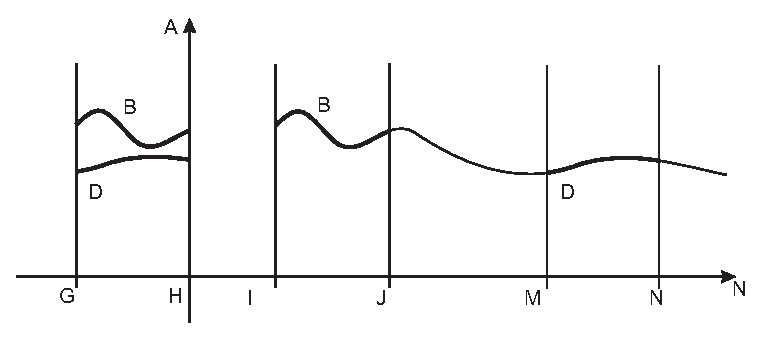
\includegraphics[width=350pt,height=150pt]{fig1}
\end{psfrags}
\end{center}
\caption{Движение, порожденное решением системы (\ref{1})}\label{fig1}
\end{figure}

%%% утверждения или условия внутри текста выделяйте курсивом
Мы предполагаем (см. рис.\,\ref{fig1}), что {\it множество попарно различных
показателей Ляпунова системы $A$ не более чем счетно и их можно упорядочить в
порядке убывания.} Расположим функции $u^1,\ldots, u^p$, образующие базис\!
%-------------------------------------
\footnotemark         % сноска (обратите внимание на \!)
\footnotetext{{\footnotesize При каждом $t$ запись $\dot L(t)$ означает .... }}
%-------------------------------------
в порядке возрастания ..........
\vspace{3pt}

\begin{teo}[о триангуляции]  \label{teor-1}
%%% обратите внимание на правильное оформление пунктов а) и б)
%%% и круглых скобок внутри текста в пункте а) (внутри окружения \it
%%% применяется окружение \rm)
{\it Если $\mathbb S^p$  вполне регулярно, то:

{\rm а)} найдутся система $B$ {\rm(}с ограниченной на $\mathbb R_+$
матрицей $B(t)${\rm)} и ляпуновское преобразование, приводящее $(A,\mathbb S^p)$ к $B$;

{\rm б)} в множестве $\{B\}$ всех систем, кинематически подобных
$(A,\mathbb S^p)$, найдется система с непрерывной и ог\-раниченной
верхней треугольной матрицей $B(t)$.}
\end{teo}

%------------------------------
\sect{Доказательство теоремы \ref{teor-1} \label{Dok}}

{\bf 1.} Еще раз поясним смысл некоторых обозначений. Зафиксируем в
подпространстве .............

{\bf 2.} Выберем пока произвольную непрерывную функцию ........

{\bf 3.} Построим теперь функцию $t\to {\widetilde B}(t)$ так, ........

Далее, из равенства ${\widehat Y}(t,0)=V(t)$ следует неравенство
\begin{gather}\label{4.1}
{\widehat Y}(t,0)|\leqslant\alpha|{V}(t)Z(t)|=\ldots=\alpha|Z(t)|
\leqslant\alpha\sqrt{r}\,\|U_t\|_{\mathbb R^p\to\mathfrak S},
\end{gather}
%%% используем \widehat вместо \hat
%%% используем \widetilde вместо \tilde
%%% используем \overline вместо \bar
%%% для многоточия используем \ldots
что и требовалось доказать. \hfill $\square$

%%% Все возможные примеры утверждений написаны ниже.
%%% В теоремах, леммах, предложениях, утверждениях, следствиях, гипотезах
%%% их содержимое выделяется курсивом {\it } с упомянутыми выше оговорками
%%% о выпрямлении скобок и прямом написании формул.
%%% В определениях курсивом выделяется только определяемое понятие.
%%% В замечаниях, примерах, предположениях, условиях содержимое курсивом не выделяется

\begin{teo} \label{teopr}
{\it Пусть выполнены условия предположения {\rm \ref{assumpr}}. Тогда ...}
\end{teo}

\begin{lem} \label{lempr}
{\it Пусть .......}
\end{lem}

\begin{pre} \label{prepr}
{\it Пусть .......}
\end{pre}

\begin{utv} \label{utvpr}
{\it Пусть .......}
\end{utv}

\begin{sle} \label{slepr}
{\it Пусть .......}
\end{sle}

\begin{hyp} \label{hyppr}
{\it Теорема {\rm \ref{teopr}} верна.}
\end{hyp}

\begin{df} \label{dfpr}
Множество $A$ называется {\it регулярным}, если ....
\end{df}

\begin{zam} \label{zampr}
Заметим, что ....
\end{zam}

\begin{pr} \label{prpr}
Рассмотрим пример ....
\end{pr}

\begin{assum} \label{assumpr}
Функции $\xi_i(t)$ являются почти периодическими в смысле Бора.
\end{assum}

\begin{cond} \label{condpr}
Начальные позиции участников таковы, что .....
\end{cond}

%----------------------------------------------
\vspace{1ex}

\makeatletter
\@fundingrus\par
\@addtoreset{equation}{section}
\@addtoreset{footnote}{section}
\renewcommand{\section}{\@startsection{section}{1}{0pt}{1.3ex
plus 1ex minus 1ex}{1.3ex plus .1ex}{}}

\vspace{3ex}
\small
{ %\scriptsize

\renewcommand{\refname}{{\rm\centerline{СПИСОК ЛИТЕРАТУРЫ}}}

\begin{thebibliography}{99}

%%%%  Не допускаются ссылки на еще не опубликованные статьи
%%%%
%%%%  ОФОРМЛЕНИЕ ЛИТЕРАТУРЫ (ВНИМАТЕЛЬНО СМОТРИМ НА ЗНАКИ ПРЕПИНАНИЯ
%%%%  И ПОРЯДОК СЛЕДОВАНИЯ ВЫХОДНЫХ ДАННЫХ)
%%%%  ОФОРМЛЕНИЕ ПРИВЕДЕНО В СООТВЕТСТВИИ С ГОСТом Р 7.0.5-2008
%%%%
%%%% Для всех статей (и других источников, при наличии) следует указывать DOI следующим образом (в виде ссылки)
%%%% https://doi.org/10.20537/vm130302
%%%% Само слово DOI не пишем
%%%% Если DOI отсутствует, следует указывать url статьи на сайте журнала, или на %%%% агрегаторах: Mathnet, Elibrary, zbmath, Elsevier, SpringerLink и др.
%%%% Ссылки долны быть проверяемы.

%%%% Если статья опубликована на русском языке, то в англоязычном списке литературы в конце выходных данных статьи нужно написать (in Russian). (NEW с 01.01.2015)
%%%% Между различными областями библиографического описания тире не ставим (NEW с 01.01.2012)
%%%% Написание пробелов между инициалами и фамилией  упростилось (NEW с 01.01.2012)
%%%% Нигде не пишутся знаки ~ (тильда) \, (backslash с запятой) (если будет необходимо, их проставит редактор)
%%%% Между инициалами пробела нет, между фамилией и инициалами один пробел
%%%% Следите за пробелами после слов: том (Т. 1), номер (№ 1), выпуск (Вып. 1), страницы (С. 1--3)!
%%%% Следите за диапазонами страниц (двойное тире)! С. 20--30
%%%% Различные элементы выходных данных разделяются точками: Год. Том. Номер. Страницы
%%%% 1991. Т. 1. № 1. С. 10--20. После символа № точка не ставится.
%%%%	
%%%% Монография:
%%%% Фамилия И.О. Название книги. Город: Издательство, Год. Страницы.

\bibitem{Kras} Красовский Н.Н. Некоторые задачи теории устойчивости движения. М.: Физматгиз, 1959. 550 с.

\bibitem{KFA} Калман Р., Фалб П., Арбиб М. Очерки по математической теории систем. М.: Едиториал УРСС, 2004. 400 с.

\bibitem{BVGN}  Былов Б.Ф., Виноград Р.Э., Гробман Д.М., Немыцкий В.В. Теория показателей Ляпунова и ее приложения к вопросам устойчивости. М.: Наука, 1966. 576 с.

\bibitem{bib35} Далецкий Ю.Л., Крейн М.Г. Устойчивость решений дифференциальных уравнений в банаховом пространстве. М.: Наука, 1970. 536 с.

%%%% Учебник или учебное пособие:
%%%% Фамилия И.О. Название учебника. Номер издания (факультативно).
%%%% Город: Издательство, Год. Страницы.

\bibitem{Kud} Фихтенгольц Г.М. Курс дифференциального и интегрального исчисления. Т. 1. М.: Наука, 1966. 608 с.

\bibitem{Dem} Демидович Б.П. Сборник задач и упражнений по математическому анализу. 10-е изд. М.: Наука, 1990. 624 с.

%%%% Ссылка на диссертацию
%%%% (Указывается организация, в которой защищена диссертация.)

\bibitem{Filip} Филиппова Т.Ф. Задачи о выживаемости для дифференциальных включений: дис. \ldots\ д-ра физ.-матем. наук / ИММ УрО РАН. Екатеринбург, 1992. 266 с.

%%%% Ссылка на автореферат диссертации
%%%% (В выходных данных указывается город, в котором защищена диссертация,
%%%% а не место печатания реферата. Наименование организации необязательно.)

\bibitem{Popova} Попова С.Н. Управление асимптотическими инвариантами линейных систем: автореф. дис. \ldots\ д-ра физ.-матем. наук. Екатеринбург, 2004. 34 с.

%%%%  Статья в журнале в центральном или зарубежном издании
%%%%  Фамилия И.О. Название статьи // Название журнала. Год. Том. Номер.
%%%%  Страницы.

\bibitem{Stokes} Stokes A. A Floquet theory for functional differential equations // Proc. Natl. Acad. Sci. USA. 1962. Vol. 48. No. 8. P. 1330--1334.
https://doi.org/10.1073/pnas.48.8.1330

\bibitem{Shim} Шиманов С.Н. К теории линейных дифференциальных уравнений с последействием // Дифференциальные уравнения. 1965. Т. 1. № 1. С. 102--116.
http://mi.mathnet.ru/de6716

\bibitem{Chernov} Чернов А.В. Об одном мажорантном признаке тотального сохранения глобальной разрешимости управляемого функционально-операторного уравнения // Известия вузов. Математика. 2011. № 3. С. 95--107.
    http://mi.mathnet.ru/ivm7249

%%%%  Статья в журнале в центральном или зарубежном издании
%%%%  Фамилия И.О. Название статьи // Название журнала. Год. Том. Выпуск.
%%%%  Страницы.
%%%%  Необходимо указывать doi статьи
%%%%  В конце адреса точка не ставится

\bibitem{Dan} Данилов Л.И. О почти периодических сечениях многозначных отображений // Вестник Удмуртского университета. Математика. Механика. Компьютерные науки. 2008. Вып. 2. С. 34--41.
https://doi.org/10.20537/vm080213

%%%%  Статья в журнале Известия Института математики и информатики Удмуртского государственного университета. Укзываем DOI, если есть.

\bibitem{Plaksin}
Гомоюнов М.И., Плаксин А.Р. Конечномерные аппроксимации конфликтно-управляемых систем нейтрального типа // Известия Института математики и информатики Удмуртского государственного университета. 2017. Т. 49. С. 111--122. \\
https://doi.org/10.20537/2226-3594-2017-49-05

%%%%  Статья в журнале Известия Института математики и информатики Удмуртского государственного университета. Если DOI нет, указываем URL  на Mathnet

\bibitem{7}
Дерр В.Я., Кинзебулатов Д.М. Об умножении обобщенных функций // Известия Института математики и информатики Удмуртского государственного университета. 2006. Вып.~2~(36). C. 43--48.
http://mi.mathnet.ru/iimi111

%%%% Депонированная статья

\bibitem{Dan2}
Данилов Л.И. О почти периодических по Вейлю сечениях многозначных отображений / УдГУ. Ижевск, 2004. 104 с. Деп. в ВИНИТИ 09.06.2004, № 981-В2004.

%%%% Тезисы докладов конференции

\bibitem{Rod} Родина Л.И., Тонков Е.Л. Почти инвариантные множества управляемых систем // Дифференциальные уравнения и топология: тез. докл. Междунар. конф., посвященной 100-летию со дня рождения Л.С. Понтрягина. МГУ. М., 2008. C. 392--393.

\bibitem{BMB} Борисов А.В., Мамаев И.С., Болсинов А.В. Топология и устойчивость динамических систем // Регулярная и хаотическая динамика: тез. докл. Всероссийской конференции. УдГУ. Ижевск, 2010. С. 11.

%%%% Статья в сборнике

\bibitem{24} Зайцев В.А. Достижимость и ляпуновская приводимость линейных управляемых систем~// Оптимизация, управление, интеллект. Иркутск: ИДСТУ СО РАН, 2005. № 2 (10). С. 76--84.

%%%%ссылки на литературу из интернета- пишем адрес

\bibitem{Bell:1980} Bell M.G. Compact ccc non-separable spaces of small weight // Topology Proceedings. 1980. Vol. 5. P. 11--25.
http://topo.math.auburn.edu/tp/reprints/v05/tp05002s.pdf

%%%% Статья в журнале Труды ИММ УрО РАН

\bibitem{BP2010} Казаков А.Л.
Применение обобщенного метода характеристических рядов при построении решения одной начально-краевой задачи для системы квазилинейных уравнений~// Труды Института математики и механики УрО РАН.
2010. Т. 16. № 2. С. 91--108.
http://mi.mathnet.ru/timm551

\bibitem{PT2009} Панасенко Е.А., Тонков Е.Л. Распространение теорем Е.А. Барбашина и Н.Н. Красовского об устойчивости на управляемые динамические системы // Труды Института математики и механики УрО РАН. 2009. Т. 15. № 3. С. 185--201.
http://mi.mathnet.ru/timm415

\bibitem{But} B\"uttiker M., Imry Y., Landauer R., Pinhas S. Generalized many-channel conductance formula with application to small rings // Physical Review B. 1985. Vol. 31. Issue 10. P. 6207--6215.
https://doi.org/10.1103/PhysRevB.31.6207

\bibitem{mirosh} Miroshnichenko A.E., Kivshar Y.S. Engineering Fano resonances in discrete arrays // Physical Review E. 2005. Vol. 72. Issue 5. 056611. 7 p.
https://doi.org/10.1103/PhysRevE.72.056611

\bibitem{Ptit} Ptitsyna N., Shipman S.P. A lattice model for resonance in open periodic wavequides // arXiv: 1101.0170v1 [math-ph]. 2010.
https://arxiv.org/abs/1101.0170v1

\bibitem{rid1} Рид M., Саймон Б. Методы современной математической физики. Т. 1. Функциональный анализ. М.: Мир, 1977. 360 c.

\bibitem{berezin} Березин Ф.А., Шубин М.А. Уравнение Шрёдингера. М.: Изд-во Московского университета, 1983. 392 с.

% указывается doi русскоязычной версии статьи

\bibitem{AG-2014} Александров Д.В., Галенко П.К. Дендритный рост с вынужденной конвекцией: методы анализа и экспериментальные тесты // Успехи физических наук. 2014. Т. 184. Вып. 8. С.~833--850.
https://doi.org/10.3367/UFNr.0184.201408b.0833

% статья в сборнике статей (книге) под редакцией

\bibitem{Lutz}
Lutz C. Description logics with concrete domains~--- a survey //
Advances in modal logic. Vol.~4~/
Balbiani~P., Suzuki~N.-Y., Wolter F., Zakharyaschev M. (Eds.).
London: King's College Publications, 2003.
P.~265--296.

% Conference paper

\bibitem{Babiarz}
Babiarz A., Banshchikova I., Czornik A., Makarov E., Niezabitowski M., Popova S. On assignability
of Lyapunov spectrum of discrete linear time-varying system with control // 2016 21st International
Conference on Methods and Models in Automation and Robotics (MMAR). IEEE, 2016. P. 697--701.
https://doi.org/10.1109/MMAR.2016.7575221

\end{thebibliography}}

\receivedrus

\contactsrus

\titleeng

\pagestyle{basestyleeng}

\refereng




%%%%  Не допускаются ссылки на еще не опубликованные статьи
%%%%
%%%%  СПИСОК ЛИТЕРАТУРЫ ЛАТИНИЦЕЙ (ВНИМАТЕЛЬНО СМОТРИМ НА ЗНАКИ ПРЕПИНАНИЯ
%%%%  И ПОРЯДОК СЛЕДОВАНИЯ ВЫХОДНЫХ ДАННЫХ)
%%%%  ОТЛИЧАЕТСЯ ОТ РОССИЙСКОГО ГОСТА
%%%%
%%%% Для всех статей (и других источников, при наличии) следует указывать DOI следующим образом (в виде ссылки)
%%%% https://doi.org/10.20537/vm130302
%%%% Само слово DOI не пишем
%%%% Если DOI отсутствует, следует указываем url статьи на сайте журнала, или на агрегаторах: Mathnet, Elibrary, zbmath, Elsevier, SpringerLink и др.
%%%% Ссылки долны быть проверяемы.
%%%%
%%%% Монография:
%%%% Фамилия И.О. Название книги транслитом (курсивом) (Перевод названия на английский),
%%%% Город: Издательство, Год, страницы.
\selectlanguage{english}
\begin{center}
REFERENCES
\end{center}
\setlength{\leftmargini}{1.8em}
\begin{enumerate}
\setlength{\itemsep}{0em}
\parskip=0pt

\item
Krasovskii N.N. {\it Nekotorye zadachi teorii ustoichivosti dvizheniya} (Some problems of the theory of stability of motion), Moscow: Fizmatgiz, 1959, 550 p.

%%%% Если иностранная книга переведена на русский язык, то оформляется так
%%%%

\item Kalman R., Falb P., Arbib M. {\it Topics in mathematical system theory}, New York: McGraw-Hill, 1969, 358~p.

Translated under the title {\it Ocherki po matematicheskoi teorii sistem}, Moscow: Editorial URSS, 2004, 400 p.

%%%% Указываются все авторы монографии, слово and перед последним автором не ставится

\item
Bylov B.F., Vinograd R.E., Grobman D.M., Nemytskii V.V. {\it Teoriya pokazatelei Lyapunova  i ee prilozhe\-niya k voprosam ustoichivosti}
(Theory of Lyapunov exponents and its application to problem of stability), Moscow: Nauka, 1966, 576 p.

% Книга, переведенная с русского на английский

\item
Daletsky Y., Krein M.G. {\it Stability of solutions of differential equations in Banach spaces}, Ann. Math. Soc. Transl., vol. 43, Providence, R.I.: American Mathematical Society, 1974, 386 p.

Original Russian text published in Daletskii Yu.L., Krein M.G. {\it Ustoichivost' reshenii differentsial'nykh uravnenii v banakhovom prostranstve}, Moscow: Nauka, 1970, 536 p.


\item
Fikhtengol'ts G.M. {\it Kurs differentsial'nogo i integral'nogo ischisleniya. Tom 1} (A course of differential and integral calculus. Vol. 1), Moscow: Nauka, 1966, 608 p.

\item
Demidovich B.P. {\it Sbornik zadach i uprazhnenii po matematicheskomu analizu} (A collection of problems and exercises in mathematical analysis), Moscow: Nauka, 1990, 624 p.

%%%% Ссылка на диссертацию
%%%% (Указывается город)

\item
Filippova T.F. {\it Problems of viability for differential inclusions},  Dr. Sci. (Phys.–Math.) Dissertation, Yekaterinburg, 1992, 266 p. (In Russian).

%%%% Ссылка на автореферат диссертации
%%%% (В выходных данных указывается город, в котором защищена диссертация,
%%%% а не место печатания реферата. Наименование организации необязательно.)

\item
Popova S.N. {\it Control over asymptotic invariants of linear systems}, Abstract of Dr. Sci. (Phys.--Math.) Dissertation, Yekaterinburg, 2004, 34 p. (In Russian).

%%%%  Статья в журнале в центральном или зарубежном издании
%%%%  Фамилия И.О. Название статьи на английском языке,
%%%%  Название журнала транслитом (курсивом), Год, том, номер, страницы (пишутся две буквы p, если страниц больше чем одна)
%%%%  Если существует перевод статьи на английский язык, то указываются выходные данные переводной статьи. Если статья имеет DOI, его необходимо указать.

\item
Stokes A. A Floquet theory for functional differential equations, {\it Proc. Natl. Acad. Sci. USA}, 1962, vol. 48,  no. 8, pp. 1330--1334.
https://doi.org/10.1073/pnas.48.8.1330

\item
Shimanov S.N. On a theory of linear differential equations with after-effect, {\it Differ. Uravn.}, 1965, vol. 1, no. 1, pp. 102--116 (in Russian).
http://mi.mathnet.ru/eng/de6716

\item
Chernov A.V. A majorant criterion for the total preservation of global solvability of controlled functional operator equation, {\it Russian Mathematics}, 2011, vol. 55, issue 3, pp. 85--95.\\
https://doi.org/10.3103/S1066369X11030108

%%%%  Статья в журнале Вестник Удмуртского университета. Математика. Механика. Компьютерные науки
%%%%  Фамилия И.О. Название статьи на английском языке, Название журнала транслитом (курсивом), Год, номер, страницы.

\item
Danilov L.I. On almost periodic selections of multivalued maps, {\it Vestnik Udmurtskogo Universiteta. Matematika. Mekhanika. Komp'yuternye Nauki}, 2008, issue 2, pp. 34--41 (in Russian).
https://doi.org/10.20537/vm080213

%%%%  Статья в журнале Известия Института математики и информатики Удмуртского государственного университета. Укзываем DOI, если есть.

\item
Gomoyunov M.I., Plaksin A.R.
Finite-dimensional approximations of neutral-type conflict-controlled systems, {\it Izvestiya Instituta Matematiki i Informatiki Udmurtskogo Gosudarstvennogo Universiteta},
2017, vol. 49, pp. 111--122 (in Russian). \\
https://doi.org/10.20537/2226-3594-2017-49-05


%%%%  Статья в журнале Известия Института математики и информатики Удмуртского государственного университета. Если DOI нет, указываем URL (eng) на Mathnet

\item
Derr V.Ya., Kinzebulatov D.M. On multiplication of generalized functions, {\it Izvestiya Instituta Matematiki i Informatiki Udmurtskogo Gosudarstvennogo Universiteta},
2006, issue 2 (36), pp.~43--48 (in Russian).
http://mi.mathnet.ru/eng/iimi111

%%%% Депонированная статья

\item
Danilov L.I. {\it On Weyl almost periodic selections of multivalued maps}, UdSU, Izhevsk, 2004, 104~p. Deposited in VINITI 09.06.2004, no. 981-B2004 (in Russian).

%%%% Тезисы докладов конференции

\item
Rodina L.I., Tonkov E.L. The almost invariant sets of controlled systems, {\it Differential Equation and Topology: Abstracts of Int. Conf. Dedicated to the Centennial Anniversary of Lev Semenovich Pontryagin}, Lomonosov Moscow State University, Moscow, 2008, pp. 392--393 (in Russian).

\item
Borisov A.V., Mamaev I.S., Bolsinov A.V. Topology and stability of dynamic systems, {\it Regulyarnaya i khaoticheskaya dinamika: tez. dokl. Vserossiiskoi konferentsii} (Regular and chaotic dynamics: abstracts of All-Russian conference), Udmurt State University, Izhevsk, 2010, p. 11 (in Russian).

%%%% Статья в сборнике

\item
Zaitsev V.A. Attainability and Lyapunov reducibility of linear control systems, {\it Optimizatsiya, upravlenie, intellekt} (Optimization, control, intelligence), Irkutsk: Institute for System Dynamics and Control Theory, Siberian Branch of the Russian Academy of Sciences, 2005, no. 2 (10), pp. 76--84 (in Russian).

%%%% ссылки на литературу из интернета- пишем адрес

\item
Bell M.G. Compact ccc non-separable spaces of small weight, {\it Topology Proceedings}, 1980, vol.~5, pp. 11--25.
http://topo.math.auburn.edu/tp/reprints/v05/tp05002s.pdf

%%%% Статья в журнале Труды ИММ УрО РАН (если ссылка дается на оригинальную статью)

\item
Kazakov A.L.
Application of the generalized method of characteristic series to the construction of a solution of an initial-boundary value problem for a system of quasi-linear equations,
{\it Trudy Instituta Matematiki i Mekhaniki UrO RAN}, 2010, vol. 16, no. 2, pp. 91--108 (in Russian). \\
http://mi.mathnet.ru/eng/timm551

%%%% Статья в журнале Труды ИММ УрО РАН (если ссылка дается на статью в переводной версии журнала)

\item
Panasenko E.A., Tonkov E.L. Extension of E.A. Barbashin’s and N.N. Krasovskii’s stability theorems to controlled dynamical systems, {\it Proceedings of the Steklov Institute of Mathematics}, 2010, vol. 268, suppl. 1, pp. 204--221.
https://doi.org/10.1134/S0081543810050159

\item
B\"uttiker M., Imry Y., Landauer R., Pinhas S. Generalized many-channel conductance formula with application to small rings,
{\it Physical Review B}, 1985, vol. 31, issue 10, pp. 6207--6215.\\
https://doi.org/10.1103/PhysRevB.31.6207

\item
Miroshnichenko A.E., Kivshar Y.S.
Engineering Fano resonances in discrete arrays, {\it Physical Review E}, 2005, vol. 72, issue 5, 056611, 7 p.
https://doi.org/10.1103/PhysRevE.72.056611

\item
Ptitsyna N., Shipman S.P. A lattice model for resonance in open periodic wavequides,  {\it arXiv: 1101.0170v1, [math-ph]}, 2010.
https://arxiv.org/abs/1101.0170v1

\item
Reed M., Simon B. {\it Metody sovremennoi matematicheskoi fiziki. I. Funktsionalnyi analiz} (Methods of modern mathematical physics, Vol. I: Functional analysis), Moscow: Mir, 1977, 360~p.

\item
Berezin F.A., Schubin M.A.
{\it Uravnenie Shredingera} (Schr\"odinger equation), Moscow:
Moscow State University, 1983, 392 p.

% указывается doi англоязычной версии статьи

\item
Alexandrov D.V., Galenko P.K.
Dendrite growth under forced convection: analysis methods and experimen\-tal tests, {\it Physics-Uspekhi}, vol. 57, issue 8, pp. 771--786.\\
https://doi.org/10.3367/UFNe.0184.201408b.0833

% статья в сборнике статей (книге) под редакцией

\item
Lutz C.
Description logics with concrete domains~--- a survey,
{\it Advances in modal logic. Vol. 4},
Eds.: Balbiani P., Suzuki~N.-Y., Wolter F., Zakharyaschev M.
London: King's College Publications, 2003, pp.~265--296.

% Conference paper

\item
Babiarz A., Banshchikova I., Czornik A., Makarov E., Niezabitowski M., Popova S. On assignability
of Lyapunov spectrum of discrete linear time-varying system with control, {\it 2016 21st International
Conference on Methods and Models in Automation and Robotics (MMAR)}, IEEE, 2016, pp. 697--701.
https://doi.org/10.1109/MMAR.2016.7575221

\end{enumerate}

\receivedeng

\contactseng


\end{document} 